%%This is a very basic article template.
%%There is just one section and two subsections.
\documentclass[12pt, a4paper]{article}

\usepackage[utf8]{inputenc} % Kodowanie UTF8
\usepackage{polski} % Wsparcie dla PL
\usepackage{listings}
\usepackage{color}
\usepackage[usenames,dvipsnames,svgnames,table]{xcolor}
\usepackage{hyperref} % dla linkowania do stron www
\usepackage[pdftex]{graphicx} % Wsparcie dla obrazkow
\usepackage{float} 
\usepackage{listings}
\usepackage{color}
\usepackage[usenames,dvipsnames,svgnames,table]{xcolor}

\begin{document}
\title{Wprowadzenie do Windows Phone 7}
\author{Marek Lewandowski}
\date{\today}

\maketitle

\abstract{Celem artykułu jest zapoznanie czytelnika z niezbędnymi
zagadnieniami platformy WP7 oraz oszczędzenie mu potencjalnych
nieprzyjemności.}

\section{Disclaimer, czyli autor się kaja}
 Nie jestem specjalistą od Windows Phone'a, ani nawet nie znam C\# w stopniu
 większym niż podstawowy. Nie przeszkodziło mi to jednak, aby w dość krótkim czasie stworzyć 5 aplikacji na
konkurs Microsoftu i upublikować je na marketplace'sie. Swoją drogą konkurs
okazał się być niewypałem, ale to już temat na inny artykuł.

Chcę tutaj przedstawić niezbędną garść informacji, tak aby móc stworzyć
aplikację, która nie obleje certyfikacji co wiąże się ze sporą
stratą czasu, bo co najmniej 1 tygodnia, co czasem może być krytyczne. Sposób w
jaki to zrobię to wskazanie czytelnikowi konkretnych tutoriali. Sam artykuł bez
przerobienia tego co znajduje się pod odnośnikami jest bez sensu. Jeśli
chciałbym umieścić wszystko tutaj to miałoby to nie kilka stron, a kilkaset co
absolutnie nie jest moim celem.

\section{Parę szybkich}
Czyli parę odpowiedzi na pytania, które możesz sobie teraz zadawać.
\subsection{Czy to coś kosztuje?}
Nie, SDK jest darmowe.
\subsection{Ile zapłacę za developerskie konto na marketplace?}
Nic, o ile jesteś studentem i skorzystasz z rejestracji przez program Microsoftu
\href{https://www.dreamspark.com/}{Dreamspark}. Od razu zaznaczę, że legitymacja
studencka nie wiele tutaj daje. Algorytm potwierdzenia statusu studenta wygląda
tak:
\begin{enumerate}
  \item Jak masz kartę ISIC to koniec, jak nie to 2.
  \item Znajdź kogoś z koła/grupy .NET żeby udostępnił Ci kod rejestracyjny, jak
  nie to 3.
  \item idź do 1.
\end{enumerate}
\subsection{Czy WP7 jest fajne?}
Tak, moim zdaniem jest całkiem niezłe, a na pewno bardzo proste do tworzenia nań
aplikacji. W miarę niezły emulator telefonu znacznie ułatwia pisanie aplikacji.
Nie jest to taki emulator jak ten do Androida, który uruchamia się minutę. Ten
jest całkiem szybki. Poza tym debugger Visuala jest chyba najlepszy, więc
pracuje się naprawdę przyjemnie. Poza tym mamy do dyspozycji takie coś jak
Expression Blender gdzie można dość łatwo składać UI i robić animację.
\subsection{\ldots serio?}
Tak, może tym razem przekona Cie to, że każdy telefon, na którym chodzi WP7 musi
zaspokajać
\href{http://msdn.microsoft.com/en-us/library/ff637514%28v=vs.92%29.aspx}{standard
 Microsoftu co do sprzętu}, więc nie trzeba pisać N wersji tej samej aplikacji,
 żeby ikonki się dobrze wyświetlały. Poza tym zakładając, że
zainteresowanie WP7 będzie rosnąć, a obecnie market jest raczej pusty to można
go opanować swoimi aplikacjami. Poza tym jest
\href{http://msdn.microsoft.com/en-us/library/ff402535%28v=vs.92%29}{MSDN} i
 można spokojnie brać przykłady metodą Copy'ego Paste'a i będą działać.

\pagebreak

\subsection{Co to jest Metro style?}
Najprościej będzie jak pokaże parę przykładów.
\begin{itemize}
   \item
	\href{http://msdn.microsoft.com/en-us/library/windows/apps/hh464920.aspx}{Tutaj 6 minutowy film wprowadzający w temat.} 
	\item
	\href{http://msdn.microsoft.com/en-us/library/windows/apps/hh974576.aspx}{Tutaj bardziej opisowo}
	\item
	\href{http://msdn.microsoft.com/en-us/library/windows/apps/hh465424.aspx}{Wskazówki
	dla tworzenia aplikacji w stylu Metro}
	\item
	\href{http://www.microsoft.com/design/toolbox/tutorials/windows-phone-7/metro/}{Filmy
	wideo i materiały}
	\item \href{http://windows.github.com/}{Przykład strony w stylu Metro}
	\item \href{http://create.msdn.com/en-US/education/basics/ux_ui}{User
	Experience and User Interface}
\end{itemize}

Tych materiałów jest bardzo dużo i w zasadzie nie ma większego sensu wszystkiego
oglądać. Jeśli przejrzałeś/przejrzałaś te linki to prawdopodobnie masz już
jakiś ogląd sytuacji.
 Sporo jest materiałów na
\href{http://channel9.msdn.com/}{channel9} i zainteresowanych odsyłam właśnie tam.

\begin{figure}[H]
		\begin{center}
		\fbox{
		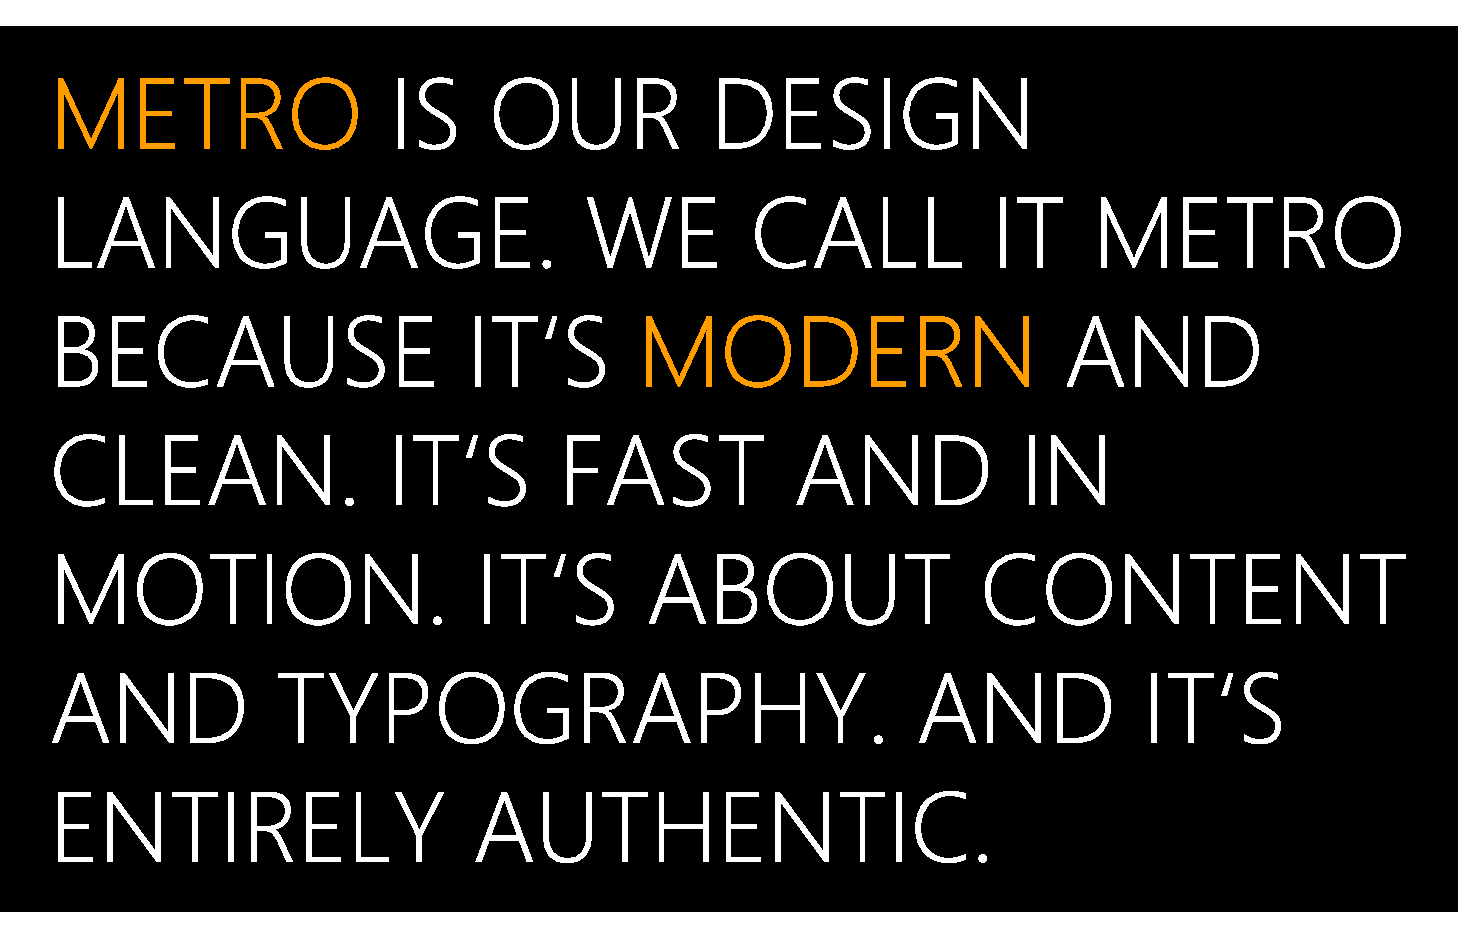
\includegraphics[width=\textwidth]{metro2.pdf}
		}
		\caption{Definicja stylu Metro}		
		
		\end{center}
\end{figure}  

\subsubsection{Gry}
Warto dodać, że wymaganie na styl Metro odnosi się głównie do aplikacji
użytkowych. Tworząc gry mamy wolną rękę przy projektowaniu menu gry i wszystkich
jej elementów.

\section{Zaczynamy}
Pierwszym krokiem jest ściągnięcie SDK. Do tego nie potrzeba żadnej rejestracji.
SDK ściągamy
\href{http://www.microsoft.com/en-us/download/details.aspx?id=27570}{stąd}.
Głęboko wierzę w to, że nawet jeśli ten odnośnik przestanie działać to sobie
poradzisz. Jeśli masz już zainstalowanego Visuala, to będziesz miał w nim
wszystko co potrzebujesz. Jeśli nie to zainstaluje Ci się wersja Express i
reszta SDK.
Jak już masz SDK to możemy pójść krok dalej.

\section{Piszemy pierwszą aplikację, a co}
Rzucimy się od razu na głęboką wodę i stworzymy naszą pierwszą aplikację.
W tym celu
\begin{enumerate}
  \item utwórz nowy projekt
  \item wybierz Visual C\#
  \item potem Silverlight for Windows Phone
  \item a na sam koniec typ aplikacji jako zwyczajną Windows Phone Application
  \item gotowe!
\end{enumerate}

To nie było trudne, prawda? Aplikacja gotowa jak się patrzy. Oczywiście żartuję,
ale w ten sposób mogę powiedzieć o typowych elementach dla każdej aplikacji na
WP7.
\subsection{Elementy aplikacji}
To co widzimy w naszym projekcie poprzez Solution Explorer to katalog
Properties, coś jak katalog o nazwie References oraz pliki źródłowe aplikacji
oraz parę podstawowych obrazków.

\subsubsection{Katalog Properties}
Tutaj znajdują się pliki manifestu i inne rzeczy, których nigdy nie będziesz
modyfikował ręcznie ponieważ tak się nie robi. Jaka kolwiek zmiana w
ustawieniach projektu powinna się odbywać poprzez klik prawym na projekt i
wybranie Properties, a tam dopiero korzystając z zakładek mamy wpływ na to co
będzie znajdowało się w plikach manifestu.

Najprzydatniejszą zakładką jest ta, która pewnie od razu Ci się pojawiła czyli
 Application. Będziesz tutaj ustawiał między innymi grafiki, które są ważne przy
 certyfikacji oraz informacje o sobie, czyli Tobie, czyli autorze w
 \emph{Assembly Information}. 
Ustawiasz tutaj także, która strona ma się pojawić po uruchomieniu
aplikacji czyli tzn. entry point. Do stron dojdziemy później.

\subsubsection{References}
To w zasadzie nie jest katalog, ale po prostu zbiór tego z czego korzysta swój
projekt. Jeśli będziesz gdzieś w kodzie dodawał np.
\lstset{language=[Sharp]C, basicstyle=\footnotesize, numbers=left,
numberstyle=\footnotesize, stepnumber=1, numbersep=10pt, breaklines=true, frame=shadowbox, rulesepcolor=\color{SkyBlue}}
\begin{lstlisting}
using Microsoft.Xna.Framework.Audio;
\end{lstlisting} 

a nie będziesz miał XNA dołączonego do projektu to Ci nie zadziała. Dla tych
którzy znają C\# jest to prawdopodobnie oczywiste.

\subsubsection{App.xaml}
App xaml oraz xaml.cs tworzą jedną całość. Jest to w zasadzie plik określający
dokładnie co się dzieje gdy włączamy naszą aplikację. Osobiście nie miałem
żadnej potrzeby modyfikowania tego pliku. Domyślną stronę, można ustawić poprzez
Properties. Myślę, że jeśli będzie taka potrzeba żeby coś tutaj zmodyfikować to
będziesz wiedzieć na tyle dużo, żeby to zrobić.

\subsubsection{Pliki.xaml i .xaml.cs}
Teraz ogólnie o plikach. Najprościej powiedzieć, że to co w xaml to widok,
a to co w xaml.cs to logika, ale było by to nie prawdą, więc powiem inaczej. To
co znajduje się w pliku xaml tworzy strukturę widoku poprzez zagnieżdżanie w
sobie elementów Silverlight'a, a cały kod i to co będzie obsługiwało stronę
znajduje się w pliku z kodem, czyli .xaml.cs. Oba pliki tworzą jedną klasę,
która jest stroną (PhoneApplicationPage).

Jeśli przyjrzysz się temu co wygenerował Visual to zobaczysz, że tworzenie UI
jest bardzo proste i przyjemne. Żeby dodawać elementy otwórz sobie Toolbox.
Znajdziesz tam podstawowe elementy jakie możesz dać. Powinieneś już znać ten
mechanizm. Warto też mieć otwartą zakładkę Properties dla danego elementu. Jest
tam dużo opcji przez, które można się przeklikać. To pewnie też już znasz z
poprzednich projektów.

Więcej o stronach w dalszej części.

\subsubsection{Architektura}
Jeśli chcesz się dowiedzieć jak działa WP7 to polecam przeczytanie
\href{http://msdn.microsoft.com/en-us/library/ff967549%28v=vs.92%29}{tych
 materiałów}. Radziłbym jednak zacząć od razu od kilku tutoriali, a dopiero
 potem wgłębiać się w szczegóły jak to wszystko działa.

\subsection{Expression Blend}
To narzędzie dołączone do SDK, które pozwala w łatwy i przyjemny sposób tworzyć
zaawansowane UI razem z animacjami i wszystkim na co pozwala Silverlight, a jest
tego dość dużo. Żeby edytować jakąś stronę wystarczy na nią kliknąć prawym i
wybrać Open in Expression Blend.

\subsection{Wrzuć to na market}
A zobaczysz, że Ci się nie uda. Nie z powodu, że tam nic nie ma i jest to
wygenerowana startowa aplikacja, ale z powodu ikonek, które jeszcze trzeba sobie
samemu zrobić. Nie można też wrzucać ikonek, które są właśnie takie domyślne.
Certyfikacje przechodzi jednak domyślny SplashScreen, więc nie wszystko trzeba
generować, ale jakby się zastanowić to kto normalny wrzucał by prawdziwą
aplikacje z jakimi kolwiek domyślnymi ustawieniami i wyglądem? W sumie to ja,
ale te aplikacje były na konkurs, więc mniejsza z tym\ldots

Najlepszym sposobem, żeby sprawdzić wszystkie takie podstawowe wymagania
odnośnie ikonek jest użycie czegoś co nazywa się \emph{Marketplace Test Kit}.
Włącza się to poprzez kliknięcie prawym na projekt, albo poprzez menu
\emph{Project}. Można tam automatycznie przetestować poprawność wszystkich
ikonek oraz poprawność zbudowanego projektu. Koniecznie wersja Release. Jest tam
też spis manualnych testów, które można wykonać. Są to te same testy, które
będzie wykonywał np. George - pracownik Microsoftu w Indiach.

\section{Proces certyfikacji}
Dokładny opis procesu certyfikacji oraz wszystkie wymagania znajdziesz tutaj
\href{http://msdn.microsoft.com/en-us/library/hh184843%28v=vs.92%29}{Application
 Certification Requirements for Windows Phone}
 
 Tych wymagań nie jest dużo, pierwsze parę stron można od razu przeskoczyć,
 ponieważ odnoszą się do praw autorskich, wulgaryzmów i innych rzeczy, których
 nie trzeba tłumaczyć.
 
 Najbardziej uciążliwym wymaganiem dla mnie stanowiło wymaganie 6.5 odnoszące
 się do nie-muzycznych aplikacji, które odtwarzają muzykę. Przykładem takiej
 aplikacji jest dowolna gra, która odgrywa sobie jakiś dźwięk w tle. Z
 przykrością muszę przyznać, że poległem pod tym wymaganiem i moja aplikacja
 NyanCat nie została certyfikowana. Choć w tym momencie nie wiele Ci to powie to
 pamiętaj, że to wymaganie odnosi się tylko do aplikacji, które używają
 \href{http://msdn.microsoft.com/en-us/library/system.windows.controls.mediaelement.aspx}{MediaElement}.
 Jeśli chcesz odtwrzać krótkie dźwięki albo nawet nie krótkie tylko takie, które nie trwają przez cały czas użytkowania aplikacji to
 należy używać czegoś co nazywa się
 \href{http://msdn.microsoft.com/en-us/library/microsoft.xna.framework.audio.soundeffect.aspx}{SoundEffect}.
 
 Przyczną tego, że poległem jest to, że nie da się tego sprawdzić na emulatorze
 ponieważ, nie da się włączyć w żaden sposób tego Zune player'a, bo go po prostu
 tam nie ma. Dlatego próba poprawienia czegoś i wrzucenia tego na Marketplace,
 po czym czekanie tydzień na wynik nie jest zbyt rozsądną opcją. Jeśli będziesz
 chciał używać MediaElement radzę Ci pożyczenie od kogoś telefonu z WP7, bo bez
 tego ciężko to sprawdzić.
 
 Poza tym sam proces certyfikacji nie jest za bardzo rygorystyczny. Jeśli
 aplikacja nie wyburacza się po 10 sekundach od jej włączenia to myślę, że
 spokojnie przejdzie ona certyfikację. Oznacza to mniej więcej tyle, że nikt nie
 sprawdza tych aplikacji pod kątem rzeczywistego działania i braku błędów. Z
 dumą mogę powiedzieć, że moje 5 słabych aplikacji, które mają teraz w sumie 3k
 ściągnięć nie zaliczyło żadnego crasha. Jest to widoczne z panelu na AppHubie,
 tak samo jak inne aktywności związane z Twoimi aplikacjami.

\section{PhoneApplicationPage}
Stroną można nazwać, każdy ekran aplikacji, który jest widoczny i do
którego można przejść, np. jeśli po urchomieniu chcesz mieć menu z przyciskiem
start, który urchomi gre to właśnie gra będzie na drugiej stronie. Najprościej
jeśli przyjmiesz, że to co oglądasz na telefonie to jest strona i możesz
pomiędzy nimi przechodzić.

Zmiana strony wygląda tak:
\lstset{language=[Sharp]C, basicstyle=\footnotesize, numbers=left,
numberstyle=\footnotesize, stepnumber=1, numbersep=10pt, breaklines=true, frame=shadowbox, rulesepcolor=\color{SkyBlue}}
\begin{lstlisting}
NavigationService.Navigate(new Uri("/NazwaStrony.xaml", UriKind.Relative));
\end{lstlisting} 

Jak widać jest to nazwa relatywna do miejsca z którego przechodzimy. Można także
używać absolutnych ścieżek, zmieniając oczywiście drugi argument.

\subsection{Dane pomiędzy stronami}
Żeby jedna strona mogła odczytać jakieś dane utworzone na drugiej stronie,
trzeba skorzystać z zapisu tych danych w ogólnie dostępne miejsce. Można
posłużyć się np. czymś co nazywa się
\href{http://msdn.microsoft.com/en-us/library/ff402541%28v=vs.92%29.aspx}{Isolated
 Storage}
Tutorial znajduje się
\href{http://create.msdn.com/en-US/education/quickstarts/Isolated_Storage}{tutaj}.
W wielkim skrócie to zapisujemy dane w formie klucz-wartość i tym samym je
odtwarzamy. Nawet jeszcze lepszy tutorial jest 
\href{http://msdn.microsoft.com/en-us/windowsphonetrainingcourse_yourfirstwp7applab_topic4#_Toc306647178}{tutaj},
ponieważ możemy ściągnąć sobie taką małą klasę IsolatedStorageHelper, która
pozwala w łatwy sposób zapisywać całe obiekty. Osobiście z tego skorzystałem.


\section{XNA}
Jeśli robimy jakąś żywszą grę to będziemy używać właśnie XNA. XNA to obszar na
osobny artykuł, ale jeśli mam coś o tym wspomnieć to po stworzeniu aplikacji
wyłącznie typu XNA to będziemy mieli wygenerowane 4 kluczowe metody oraz
zostanie zainicjowany timer gry, który będzie cykał i wołał w odpowiednim czasie
metody do rysowania oraz odświeżenia logiki.

Metody to:
\begin{itemize}
  \item OnNavigatedTo - ładowanie zasobów, start timera
  \item OnNavigatedFrom - zwalnianie zasobów, stop timera
  \item OnUpdate - odświeżenie stanu gry, tutaj powinna być logika
  \item OnDraw - rysowanie, wizualizacja stanu gry
\end{itemize}

Możliwości XNA są ogromnę i nie jestem w stanie ich tutaj opisać, chociażby z
powodu, że poznałem XNA tylko w bardzo małym stopniu.

\section{I'm mixin it, czyli Silverlight \& XNA}
Podczas tworzenia gry zazwyczaj menu będzie robione używając gotowych
kontrolek, a reszta gry będzie działała pod udziałem XNA.
Możliwe jest także łączenie tych dwóch technik. Wtedy Silverlight jest renderowany jako tekstura i
wyświetlany razem z innymi teksturami. 
\href{http://msdn.microsoft.com/en-us/library/hh202938%28v=vs.92%29}{Tutorial
 tutaj}

\section{Różne elementy WP7}
Mógłbym tutaj przepisywać treść tutoriali z msdn, ale myślę, że nie ma to
większego sensu dlatego też wskazuję miejsce gdzie należy szukać informacji i
gdzie znajdują się bardzo dobre tutoriale dotyczące różnych mechanizmów WP7.
\href{http://msdn.microsoft.com/en-us/library/ff431744%28v=vs.92%29.aspx}{Tutoriale
 tutaj}.

\section{Słowo końcowe}
Celem tego artykuły było to, żebyś czytelniku wiedział gdzie masz dalej szukać
informacji i miał już pewien minimalny poziom informacji od czego zacząć i
czego się spodziewać. Celowo nie przygotowałem własnego fragmentu kodu, ponieważ
te na MSDN są zbyt dobre, żeby z nich nie korzystać. Jeśli będziesz czegoś
szukał kieruj się właśnie tam.\\
Powodzenia.
\\\\\\
\emph{Użyteczne linki}:\\
\href{http://msdn.microsoft.com/en-us/library/ff402535%28v=vs.92%29}{Windows
 Phone Development}\\
\href{http://create.msdn.com/en-US/}{AppHub}\\
\href{https://www.dreamspark.com/}{Dreamspark}\\
\href{http://www.codeguru.pl/}{Codeguru}\\
\href{http://channel9.msdn.com/Series/Kurs-programowania-Windows-Phone-7}{Kurs
programowania Windows Phone 7}\\


\end{document}
